%
%H27 修士論文中間発表用予稿
%
\documentclass[10pt, twocolumn, a4j]{jsarticle}
\usepackage{enumerate}
\usepackage{subfigure}
\usepackage[dvips]{graphicx}
\usepackage{amsmath,amssymb,amsfonts}
\usepackage[varg]{txfonts}
\usepackage{mediabb}%PDF図添付
\usepackage{cite}

\pagestyle{empty}
\renewcommand{\baselinestretch}{0.75}
\renewcommand{\rmdefault}{ptm}
\setlength{\textwidth}{175mm}
\setlength{\textheight}{261.9mm}
\setlength{\oddsidemargin}{-7.9mm}
\setlength{\evensidemargin}{-7.9mm}
\setlength{\topmargin}{-7.9mm}
\setlength{\headheight}{0mm}
\setlength{\headsep}{0mm}
\setlength{\footskip}{0mm}
\setlength{\textfloatsep}{3mm}

\begin{document}

\setlength{\abovedisplayskip}{3pt} % 数式と本文の上部のマージン
\setlength{\belowdisplayskip}{3pt} % 数式と本文の下部のマージン
\setlength\textfloatsep{3pt} %図と本文の間の余白調整
\makeatletter
%\def\section{\@startsection{name}{level}{indent}{beforeskip}{afterskip}{style}}
%\def\subsection{\@startsection {subsection}{1}{\z@}{-3.5ex plus -1ex minus -.2ex}{2.3 ex plus .2ex}{\normalsize\bf}}
\def\section{\@startsection {section}{1}{\z@}{3 ex}{1ex}{\large\bf}}
\def\subsection{\@startsection {subsection}{1}{\z@}{3ex}{1ex}{\normalsize\bf}}
\def\subsubsection{\@startsection {subsubsection}{1}{\z@}{1ex}{1ex}{\normalsize\bf}}
\newcommand{\Max}{\mathop{\rm max}\limits}
\makeatother
% --------------------------------------------------------------------- %
\twocolumn[
  %% \begin{flushright}
  %%   \vspace{-7mm}
  %%   \small 特許出願予定につき非公表
  %% \end{flushright}
  \begin{center}
    % header
    {\small 平成27年度 電気通信大学大学院 情報・通信工学専攻 ICコース 修士論文発表会 AWCC藤井研究室予稿}\\
    \vspace{1zw}
    % title
    {\bf \Large プライマリの時間的通信状況を考慮した電波環境データベース構築}\\
    \vspace{1zw}
    %author
    {\small 発表者 1431019 王 昊, 主任指導教員 : 藤井 威生 教授, 指導教員 : 山尾 泰 教授}\\
    {\small 先端ワイヤレス・コミュニケーション研究センター 藤井研究室}
    \vspace{1zw}
    %連絡先
    %\normalsize{\itshape{
    %Advanced Wireless and Communications research Center (AWCC) \\
    %The University of Electro-Communications \\
    %1-5-1 Chofugaoka, Chofu, Tokyo, 182-8585 Japan \\
    %TEL:042-443-5917, FAX:042-443-5860 \\
    %○○○○@awcc.uec.ac.jp
    %}}
  \end{center}
]

\section{はじめに}
コグニティブ無線\cite{Haykin}を用いた周波数共用において,周波数の二次利用者(SU: Secondary User)は既存の周波数割り当てユーザ(PU: Primary User)への干渉を回避する必要がある.その中で自身の通信品質を確保するためには,正確な電波環境推定技術が重要である.現在,実用的な電波環境推定技術として電波環境データベースに注目を集めている.SUはデータベースに予め保存されるPUからの受信電力値に関する空間的な分布といった情報を取得することにより電波環境認識を行う.これまで車載無線機やスマートフォンといった移動端末が観測した膨大な電波環境情報から各位置における周波数の利用状況を高精度に構築される電波環境データベースが提案されている\cite{DB}.
テレビ帯域を対象とした実証実験により,従来の距離減衰モデルに基づく手法と比較してPUの平均受信電力値の空間的な分布を精度良く推定できることを明らかにしている.しかし,無線LANのように観測期間内に状態遷移する可能性のあるシステムについては,最終的な平均結果とON状態のみを抽出した平均受信電力値に差が生じる恐れがあった.
そこで本研究では,観測期間内にPUの通信状態が遷移する場合の電波環境データベースの構築について検討を行う.1回の観測期間内での受信電力に関する分布変化を検出することにより,PUの通信状態の遷移点を検出するアルゴリズムを提案する.検出した遷移点を用いて、通信を行なっている状態のみの受信電力値の取り出しが可能となり,PUが通信を行なっている状態での平均受信信号電力値を精度良く推定できる.ここでは特に,有効期間の検出に焦点を当てたシミュレーション評価を行ない,その有効性を示す.
\section{システムモデル}
図1に本研究で想定するシステムモデルの概要を示す.本研究では,ONとOFFの2状態遷移するPUが1台ある環境において観測センサ1台が観測を行うこととする.観測センサは観測期間内に$T$サンプルを取得する.PUの時間的通信状態が遷移するため,観測センサが取得したサンプル$y[i]$は式(\ref{sample})のようになる.
\begin{align}
y[i]=
\left\{
\begin{array}{ll}
w[i], & i=1,\dots,\tau_1-1 \\
x[i]+w[i],& i=\tau_1,\dots,\tau_2-1 \\
w[i],& i=\tau_2,\dots,T 
\end{array}
\right.
\label{sample}
\end{align}
$\tau_1$と$\tau_2$はそれぞれOFF$\rightarrow$ONの遷移点(立ち上がり点)とON$\rightarrow$OFFの遷移点(立ち下がり点)である.また,$x[i]$はPUの送信信号で,$w[i]$は平均0,分散$\sigma^{2}$の加法性白色ガウス雑音(AWGN:Additive White Guassian Noise)である.次に,$P$は観測センサにおける受信電力値とする時,PUがOFFとONの時のサンプル値はそれぞれ平均0,分散$\sigma^2$と$\sigma^2+P$の正規分布に従うことを仮定し,確率密度関数(PDF: Probability Density Function)は式(\ref{normal})である.

\begin{align}
\begin{cases}
\;f_0(t) = \frac{1}{\sqrt{2\pi\sigma^2}} \rm{exp}^{-\frac{t^2}{2\sigma^2}} \\
\;f_1(t) = \frac{1}{\sqrt{2\pi(\sigma^2+P)}} \rm{exp}^{-\frac{t^2}{2(\sigma^2+P)}}
\end{cases}
\label{normal}
\end{align}

\begin{figure}[t]
\centering
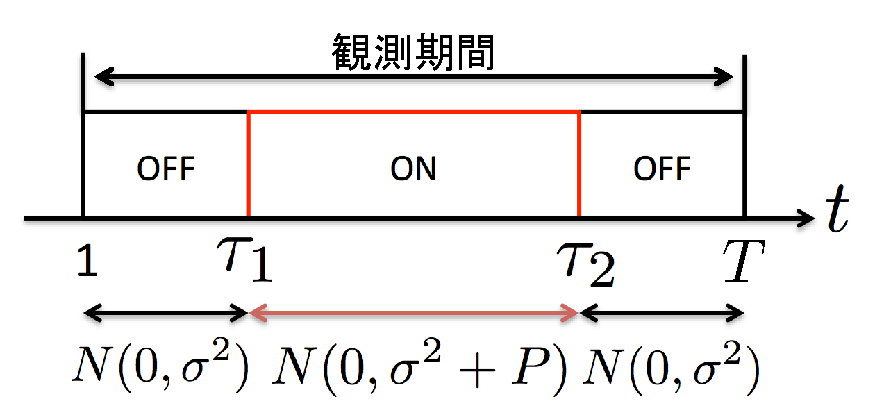
\includegraphics[clip,width=45mm]{systemodel.eps}
\caption{システムモデル}
\label{Systemmodel}
\end{figure}

\section{遷移点検出による有効期間検出}
取得した遷移点込みの全サンプルを一意に平均化を行う場合,真の電力値と差分が生じる問題がある.これに対し,OFFからONまたはONからOFFに一回しか遷移しない場合の遷移点検出法が検討されていた\cite{Quickest_detection}.本研究ではONとOFFの遷移が複数ある環境を想定した遷移点検出法を提案する.
提案手法では雑音の分散$\sigma^2$が既知で,受信電力値$P$がそれぞれ既知と未知の場合のCUSUM(cumulative sum)とGLR(Generalized Likelihood Ratio)アルゴリズムを用いて遷移点を検出する.分布が既知であるため,ONのPDF対OFFのPDFの対数尤度比$l_{1}(y[i])$を式(\ref{like})で定義する.
\begin{align}
l_{1}(y[i]) &= {\rm ln}\left\{\frac{f_1(y[i])}{f_0(y[i])}\right\} \label{like} \\
&=\frac{Py^2[i]}{2(P+\sigma^2)\sigma^2} + \frac{1}{2}{\rm ln}\left\{\frac{\sigma^2}{P+\sigma^2}\right\} \nonumber
\end{align}

OFFとONのみのサンプル値の平均対数尤度比をそれぞれ計算すると,以下の式(\ref{D_f0})と(\ref{D_f1})になる.
\begin{eqnarray}
E_{f_0}\left\{l_1(y[i])\right\} &=\int f_0(y){\rm ln}\left\{\frac{f_1(y)}{f_0(y)}\right\}dy=-D(f_0||f_1)\leq 0 \label{D_f0} \\
E_{f_1}\left\{l_1(y[i])\right\} &=\int f_1(y){\rm ln}\left\{\frac{f_1(y)}{f_0(y)}\right\}dy=D(f_1||f_0)\geq 0 \label{D_f1}
\end{eqnarray}
ここで,$D(f_0||f_1)$と$D(f_1||f_0)$は$f_0$の$f_1$と$f_1$の$f_0$に対するカルバック・ライブラー情報量である.式(4)と(5)をみると,OFFの時のサンプルの対数尤度比は負であり,ONの場合は正である.同様に計算すると,OFFのPDF対ONのPDFの対数尤度比$l_{0}(y[i])$はONの時のサンプルの対数尤度比は負であり,OFFの場合は正である.

\subsection{CUSUMアルゴリズム($\sigma^2$既知,$P$既知)}
式(\ref{D_f0})(\ref{D_f1})の性質を利用すると,対数尤度比の累積和が最大となるように式(\ref{Cusum})を遷移点の判定式として定義する.
\begin{eqnarray}
g_t =  \Max_{k \leq t}\left\{\sum_{i=1}^tl(y[i]-\sum_{i=1}^kl(y[i]))\right\}=\Max_{k \leq t}\sum_{i=k+1}^tl(y[i])
\label{Cusum}
\end{eqnarray}
$g_t$がある閾値$h$より大きい場合,分布の変化いわばPUの状態遷移発生として検出する.また$P$は既知であるため,$g_t$を式(\ref{rec})のように再帰的に計算可能である.
\begin{eqnarray}
g_{t+1}=\left\{g_t+l(y[t+1]),0\right\}^{+}
\label{rec}
\end{eqnarray}

\subsection{GLRアルゴリズム($\sigma^2$既知,$P$未知)}
$P$が常に既知とは限らないため,ここでは$P$は$[P_{{\rm min}},P_{{\rm max}}]$にあると仮定し,$g_t$の計算は式(\ref{Glr})に従う.
\newpage
\begin{eqnarray}
g_t &= \Max_{k \leq t}\sum_{i=k+1}^tl(y[i])={\rm ln}\left\{\prod_{i=k+1}^k\frac{f_{1,P}(y[i])}{f_0(y[i])}\right\} \\ 
    &= \Max_{k \leq t}\sum_{i=k+1}^t\left\{ \frac{Py^2[i]}{2(P+\sigma^2)\sigma^2}+\frac{1}{2} {\rm ln}\left\{ \frac{\sigma^2}{P+\sigma^2}\right\} \right\} 
\label{Glr}
\end{eqnarray}

また,再帰的に計算するのは不可能であるため,以下の式(\ref{fp})として$f(P)$を定義する.
\begin{eqnarray}
f(P) = \frac{P}{2(P+\sigma^2)\sigma^2}\hat{y}+(t-k)\frac{1}{2}{\rm ln}\left\{ \frac{\sigma^2}{P+\sigma^2} \right\} 
\label{fp}
\end{eqnarray}
ここで,$\hat{y}=\sum_{i=k+1}^t y^2[i]$である.次に,範囲$[P_{{\rm min}},P_{{\rm max}}]$内に$f(P)$が最大となる$P$を以下の式(\ref{maxP})によって決定する.

\begin{equation}
P^{*}=
\left\{
\begin{array}{ll}
P_{{\rm max}}, & (t-k)\leq\frac{\hat{y}}{P_{{\rm max}}+\sigma^2}, \\
\frac{\hat{y}}{t-k}-\sigma^2, & \frac{\hat{y}}{P_{{\rm max}}+\sigma^2}\leq(t-k)\leq\frac{\hat{y}}{P_{{\rm min}}+\sigma^2}, \\
P_{{\rm min}}, & (t-k) \geq \frac{\hat{y}}{P_{{\rm min}}+\sigma^2}.
\end{array}
\right.
\label{maxP}
\end{equation}
式(\ref{maxP})によって得られた$P^{*}$より式(\ref{Glr})に従い,$g_t$を計算することが可能である.

\subsection{有効期間検出}
次に,提案手法におけるONとなる有効期間の検出手順を以下の通りに示す.
\begin{itemize}
 \item[i.] 各サンプルの対数尤度比$l_1(y[i])$と$l_0(y[i])$を計算する.
 \item[ii.] CUSUMとGLRアルゴリズムにおける$g_t$の計算をそれぞれ式(\ref{Cusum})と式(\ref{Glr})に従う.
 \item[iii.] ${\rm min}\left\{t:g_t\geq h\right\}$を満たす$t_a$を遷移点として検出する.
\end{itemize}
また,図\ref{Transition}に示したようにCUSUMとGLRアルゴリズムを用いて計算した$g_t$からピーク値を検出し,それに対応するサンプルIDを遷移点として報告する.

最後に,観測センサは検出した遷移点に基づいてONのみの区間の電力値を抽出し,データベースに報告する.
\section{シミュレーション評価}
提案手法の有効性を示すために,計算機シミュレーションを行った.シミュレーション諸元を表\ref{parameter}に示す.図\ref{Powdiff}に信号対雑音比(SNR: Signal-to-Noise Ratio)を変化させた時に,検出した立ち上がり点と立ち下がり点によってON区間を抽出した電力値$P_{{\rm ON}}$と真の電力値$P$との差分$P_{{\rm diff}}$の特性を示す.ここで,$P_{{\rm diff}}$は式(\ref{diff})によって与えられる.
\begin{eqnarray}
P_{{\rm diff}} &= P-P_{{\rm ON}}
\label{diff}
\end{eqnarray}

また,従来手法としてPUの通信状態の遷移を考慮せず,全サンプルを一意に平均化を行なった場合の特性を示す.提案手法を用いることで,低SNR領域では従来手法と比較し約0.5{\rm dB},高SNR領域では約1.3{\rm dB}の低減を実現した.

%\begin{align}
%\begin{cases}
%\;{\rm CUSUM}:\bar{T_0} \geq e^h,\\
%\;{\rm GLR}:\bar{T_0} \geq \frac{1}{a}
%\end{cases}
%\end{align}


\section{まとめ}
 高精度な電波環境データベース構築に向け,PUの通信状態の時間的な変化を考慮した遷移点検出による有効期間検出法を検討した.シミュレーション評価により,提案手法を用いることで,センシング期間内に通信状態の遷移が生じる環境においても受信信号電力を精度よく推定でき,電波環境データベースの信頼度の向上を示した.
%今後の予定としては,GLRアルゴリズムにおいては$P$はある固定の範囲$[P_{{\rm min}},P_{{\rm max}}]$で遷移点検出を行ったが,フェージングやシャドウイングといった電波環境の変化に応じて範囲を適応的に変化させることによって検出性能の向上を目指す.

\begin{table}[t]
\begin{center}
 \caption{シミュレーション諸元}
 \normalsize
  \begin{tabular}{c|c}\hline
    SNR & 0〜20[dB] \\
    $[P_{{\rm min}},P_{{\rm max}}]$ & [P/2,2P] \\
    $\sigma^2$ & 1 \\
    サンプル数 & 2048 \\
   % $\bar{T}_0$ & 10 \\
    遷移パターン & OFF $\rightarrow$ ON $\rightarrow$ OFF \\
    立ち上がり点 & 512th sample\\
    立ち下がり点 & 1536th sample\\
    試行回数 & 10,000 \\ \hline
  \end{tabular}
\label{parameter}
\end{center}
\end{table}
\begin{figure}[t]
		\begin{tabular}{c}
			%1%
			\begin{minipage}{0.50\hsize}
				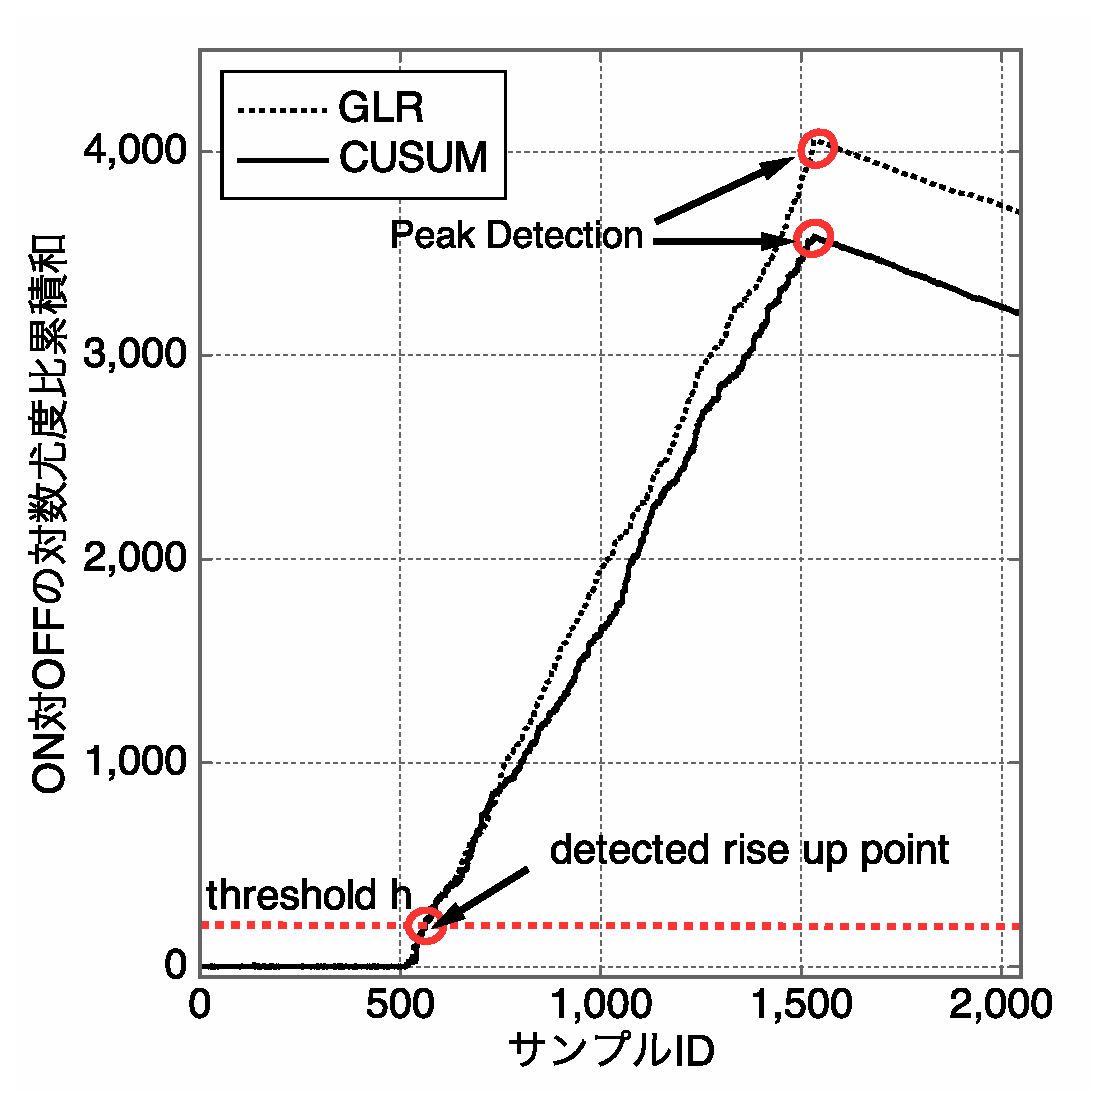
\includegraphics[clip,width=43mm,height=52mm]{OFF2ON.eps}
			\end{minipage}
			%2%
			\begin{minipage}{0.20\hsize}
				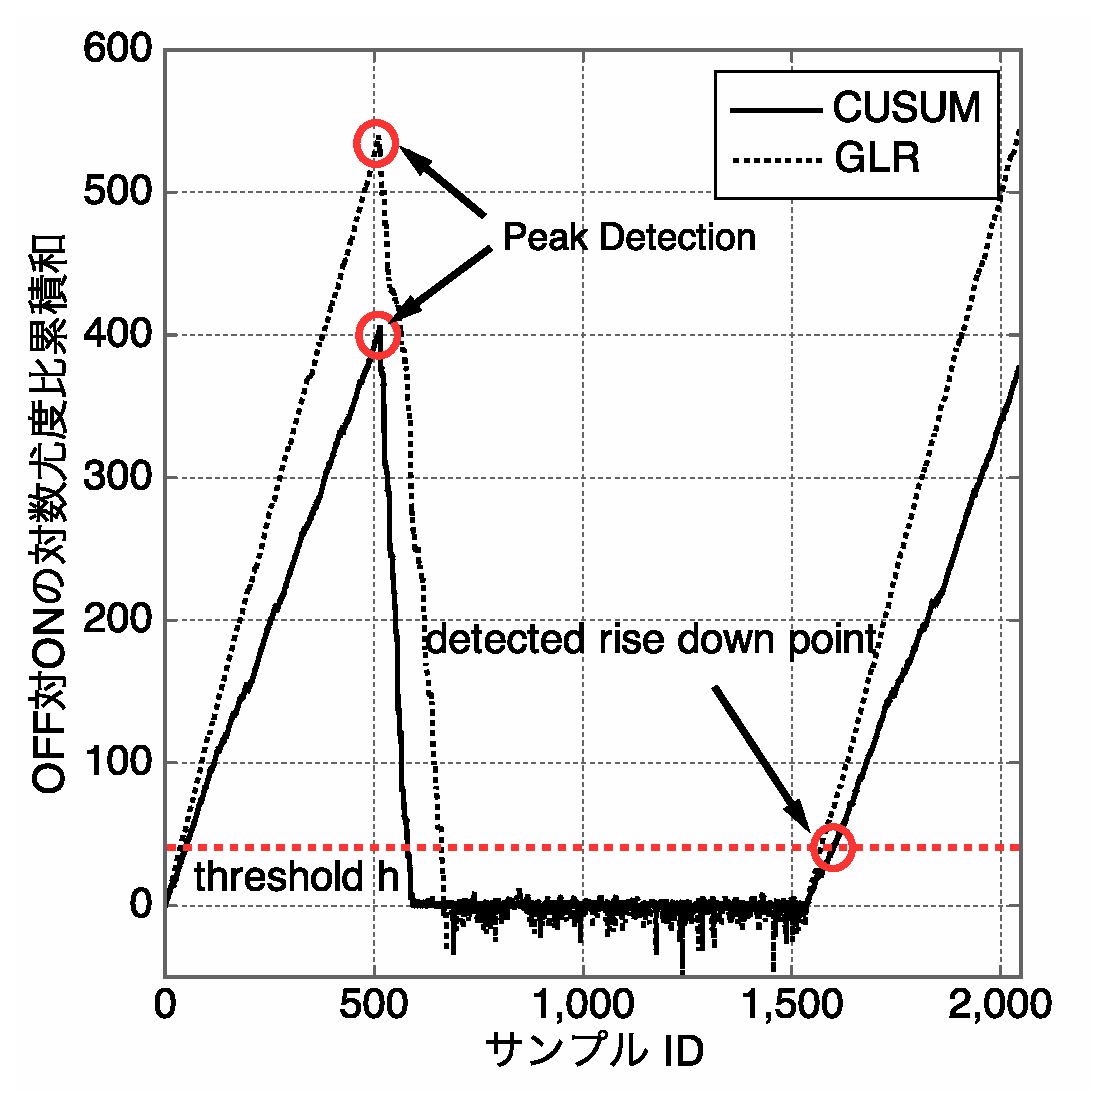
\includegraphics[clip,width=43mm,height=52mm]{ON2OFF.eps}
			\end{minipage}
		\end{tabular}
                \caption{対数尤度比累積和}
                \label{Transition}

\end{figure}
		

\begin{figure}[t]
\centering
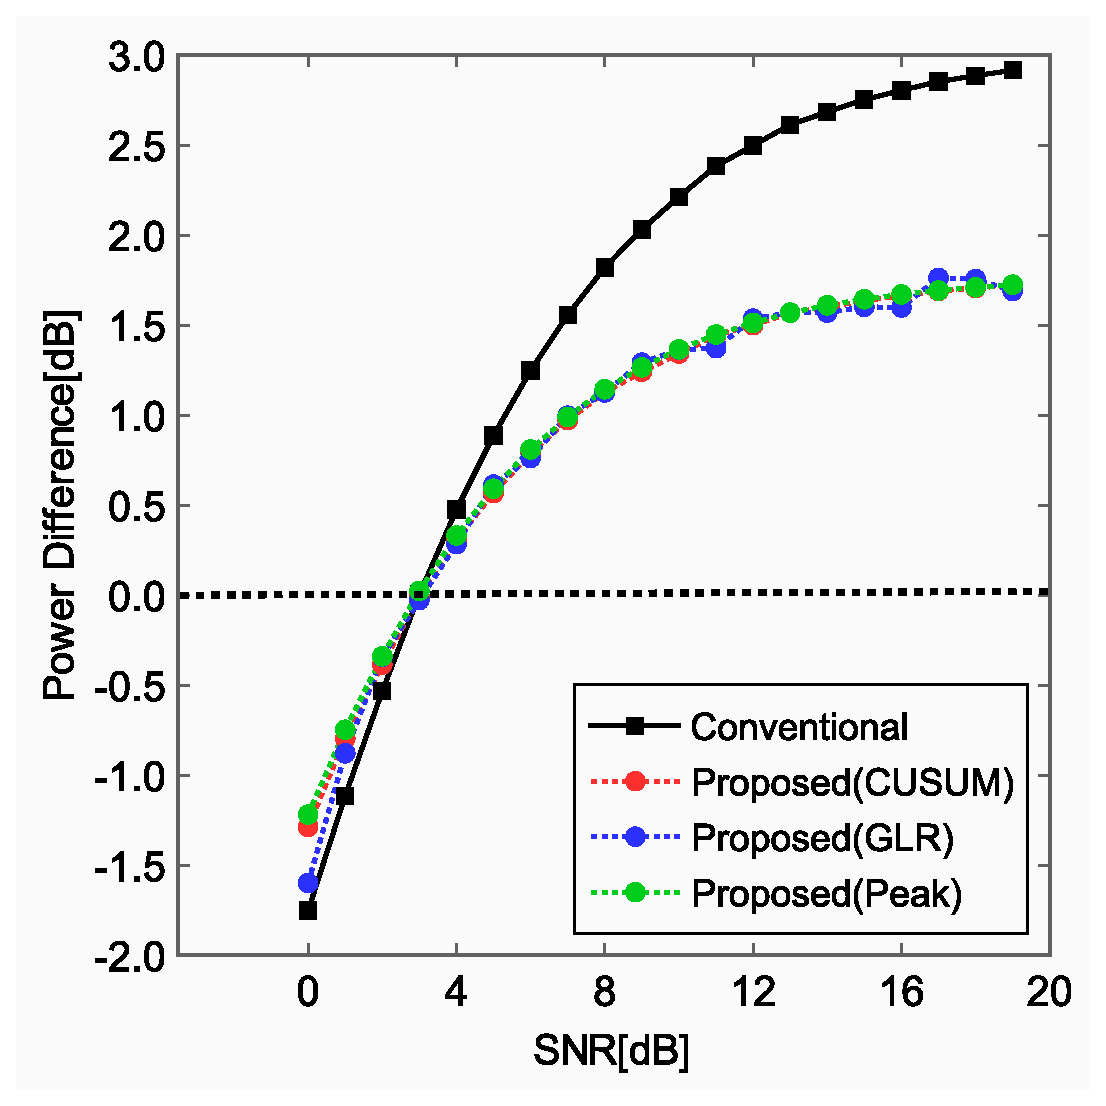
\includegraphics[width=78mm]{peak.eps}
\caption{真の電力値との差分}
\label{Powdiff}
\end{figure}

\begin{thebibliography}{9}
  \scriptsize{
  \bibitem{Haykin} S. Haykin, ``Cognitive radio: Brain-empowered wireless communications,'' {\it IEEE J.Selected Areas Commun.},vol. 23, no. 2, pp. 201 - 220, Feb. 2005.

  \bibitem{DB} K. Sato, M. Kitamura, K. Inage, and T. Fujii, ``Measurement-based spectrum database for flexible spectrum management,'' IEICE Trans. Commun., vol.E98-B, no.10, pp.2004-2013, Oct. 2015.
  \bibitem{Quickest_detection} L.Lai, Y.Fan, and H.V.Poor, ``Quickest Detection in Cognitive Radio: A Sequential Change Detection Framework,'' Proc. IEEE Globecom, Dec. 2008.
  }
\end{thebibliography}
\vspace{-5mm}
\section*{発表実績}
\noindent
\scriptsize{
  \begin{enumerate}[{[}A{]}]
  \bibitem{cite1}
    王昊,中川洸佑, 北村優行,藤井威生, ``重み付け協調センシングを用いた無線環境データベースによる状態遷移検出法,'' 信学総大, B-17-19,March 2014.
  \bibitem{cite2}
    H.Wang, T.Fujii, ``Transition detection with Spectrum Database Using Weighted Cooperative Sensing,'' Proc. IEEE ICUFN, July. 2014.
  \bibitem{cite3}
    王昊,  藤井威生, ``重み付け協調センシングおよび電波環境データベースを用いたプライマリユーザの状態遷移検出法の一検討,'' 信学技報 SR2015-1, May 2015.

他,主著3件(内査読付き国際会議論文1件,国際ワークショップ1件)\\
共著3件(内査読付き国際会議論文1件),計9件.
  \end{enumerate}
}

\end{document}
